\begin{tcolorbox}[breakable,colback=blue!5!white,colframe=blue!75!black,
 title= 判断题]

无噪声信道的容量是 $ \log a $,其中 $ a $ 是输入字母表的大小.
\tcblower
对. 无噪声信道等价条件是, 存在一个 $ \mathscr{U} \rightarrow \mathscr{V} $ 的 $ 1-1 $ 映射 $ \phi $, 使得 $ p(\phi(u) \mid u)=1 $ 对所有 $ u $ 成立, 从而 $ a=b $. 因此 $ C=\log a=\log b $.
\end{tcolorbox}



\begin{tcolorbox}[breakable,colback=blue!5!white,colframe=blue!75!black,
 title= 判断题]

无用信道的容量是 0 .
\tcblower
对.  无用信道意味着输出不依赖于输入,或者说输出对于输入的选择完全没有信息.在这种情况下,无论输入是什么,输出的分布都保持不变,因此 \(H(\eta | \xi) = H(\eta)\). $ I(\xi ; \eta)=H(\xi)-H(\xi \mid \eta)=H(\xi)-H(\xi)=0 $. (注意 $ \xi $ 与 $ \eta $ 是相互独立的.)
\end{tcolorbox}

\begin{tcolorbox}[breakable,colback=blue!5!white,colframe=blue!75!black,
 title= 判断题]

无丢失信道的容量是 $ \log a $, 其中 $ a $ 是输入字母表的大小.
\tcblower
对.  因  $\xi$  完全由  $\eta$决定,即 $ H(\xi \mid \eta)=0 $.
$$
\begin{aligned}
I(\xi ; \eta)  =H(\xi)-H(\xi \mid \eta)  =H(\xi)-0  =H(\xi) \leq \log a
\end{aligned}
$$
$ H(\xi) $ 的最大值 $ \log a $.
\end{tcolorbox}

\begin{tcolorbox}[breakable,colback=blue!5!white,colframe=blue!75!black,
 title= 解答题]

写出二元对称信道的信道矩阵, 并利用信道容量的定义求它的信道容量.
\tcblower

记输入输出字母表 $ \mathscr{U}=\mathscr{V}=\{0,1\} $. 信道转移概率分布为
$$
p(0 \mid 1)=p(1 \mid 0)=p, p(0 \mid 0)=p(1 \mid 1)=1-p
$$
则二元对称信道的信道矩阵如下所示:
$$
\begin{array}{ccc}
 & 0 & 1 \\
0 & 1-p & p \\
1 & p & 1-p
\end{array}
$$
下面利用信道容量的定义求它的信道容量. 
$$C=\max \left\{I(\xi ; \eta) \mid \xi \in \mathscr{P}_{\mathscr{U}}\right\}=\max \left\{H(\eta)-H(\eta \mid \xi) \mid \xi \in \mathscr{P}_{\mathscr{U}}\right\}$$

设入口分布为 $\left(p_{0}, p_{1}\right)$, 对应的出口分布为 $\left(q_{0}, q_{1}\right)$,则
$$
\begin{aligned}
\left(q_{0}, q_{1}\right) & =\left(p_{0}, p_{1}\right)\left(\begin{array}{cc}
1-p & p \\
p & 1-p
\end{array}\right) =\left(p_{0}(1-p)+p_{1}  p,\quad p_{0} p+p_{1}(1-p)\right)
\end{aligned}
$$
不妨设 $p_{0}=\theta ,$ 则 $ p_{1}=1-\theta, 0 \leqslant \theta \leqslant 1 $.
$$ \begin{aligned} q_{0} & =\theta(1-p)+(1-\theta) p=\theta+p-2 \theta p \\ q_{1} & =\theta p+(1-\theta)(1-p)=1-\theta-p+2 \theta p \\ H(\eta) & =-q_{0} \log _{2} q_{0}-q_{1} \log _{2} q_{1} \\ & =-q_{0} \log _{2} q_{0}-\left(1-q_{0}\right) \log _{2}\left(1-q_{0}\right) \\ & =H\left(q_{0}\right)\end{aligned} $$

 根据熵函数的性质$q_{0}$ 取$\frac 12$ 时 $H(\eta) $最大且取值为 $1$, 此时 $q_0= \theta+p-2 \theta p=\frac{1}{2} $, 化简即得 $ \theta=\frac{1}{2} $.

由于
$$
\begin{aligned}
H(\eta \mid \xi=0) & =p(0 \mid 0) \log \frac{1}{p(0 \mid 0)}+p(1 \mid 0) \log \frac{1}{p(1 \mid 0)} \\
& =(1-p) \log \frac{1}{1-p}+p \log \frac{1}{p}=H(p) \\
H(\eta \mid \xi=1) & =p(0 \mid 1) \log \frac{1}{p(0 \mid 1)}+p(1 \mid 1) \log \frac{1}{p(1 \mid 1)} \\
& =p \log \frac{1}{p}+(1-p) \log \frac{1}{1-p}=H(p) .
\end{aligned}
$$
所以
$$H(\eta \mid \xi)=\sum_{u \in \mathscr{U}} p(u) H(\eta \mid \xi=u)=\sum_{u \in \mathscr{U}} p(u) H(p)=\left(\sum_{u \in \mathscr{U}} p(u)\right) H(p)=H(p)$$

因此二元对称信道的信道容量为
$$C=\max \left\{H(\eta)-H(\eta \mid \xi) \right\}=1-H(p)$$

\end{tcolorbox}



\begin{tcolorbox}[breakable,colback=blue!5!white,colframe=blue!75!black,
 title= 解答题]

考虑离散无记忆信道 $ Y=(X+Z) \bmod 11 $, 其中
$$
Z=\left(\begin{array}{ccc}
1 & 2 & 3 \\
\frac1 3 & \frac1 3 &\frac1 3
\end{array}\right)
$$
$ X \in\{0,1, \cdots, 10\} $. 假设 $ X $ 和 $ Z $ 独立.\\
(1) 求这个信道的容量.\\
(2) 找出达到信道容量的入口分布.
\tcblower

(1) $ Y=(X+Z) \bmod 11 $, 输入为 $ X $, 输出为 $ Y, Z $ 为噪声信道, 而
$
Z=\left(\begin{array}{ccc}
1 & 2 & 3 \\
\frac1 3 & \frac1 3 & \frac1  3
\end{array}\right), \quad X \in\{0,1, \cdots, 10\}.
$
所以 $ Y \in\{0,1, \cdots, 10\} $, 

因为 $ Z $ 可以取三个值 $ (1,2,3) $ ,每个都有 $ \frac{1}{3} $ 的概率,所以对于每个 $ X $ 的值, $ Y $ 可以是三个可能的结果之一,这取决于 $ Z $ 的值.信道矩阵 $ P(Y \mid X) $ 将具有 11 行 (对应于 $ X $ 的可能值) 和 11 列(对应于 $ Y $ 的可能值).每个元素 $ P_{i j} $ 表示给定输入 $ X=i $ 时输出 $ Y=j $ 的概率.

由于 $ Z $ 的作用是加在 $ X $ 上然后对 11 取模,每个 $ X $ 值将映射到三个不同的 $ Y $ 值,每个的概率都是 $ \frac{1}{3} $ .例如,如果 $ X=0 $ ,则 $ Y $ 可以是 $ 1 , 2 $ 或 3 ,每个都有 $ \frac{1}{3} $ 的概率,因为 $ Z $ 分别加 $ 1 , 2 $ 或 3 .因此,信道矩阵的一般形式将是每行有三个 $ \frac{1}{3} $ 的条目,分别对应于 $ X $ 加上 $ 1 , 2 , 3 $ 和模 11 的结果,而其他位置为 0 .对于 $ X=0: Y $ 的可能值是 $ 1,2,3 $ ,每个概率为 $ \frac{1}{3} $ . 对于 $ X=1: Y $ 的可能值是 $ 2,3,4 $ ,每个概率为 $ \frac{1}{3} $ .以此类推,直到 $ X=10 $ .每行的具体值会随着 $ X $ 的增加而“滚动”,并在达到 10 并绕回 0 时循环.这种模式的重复构成了完整的信道矩阵:

\begin{center}
     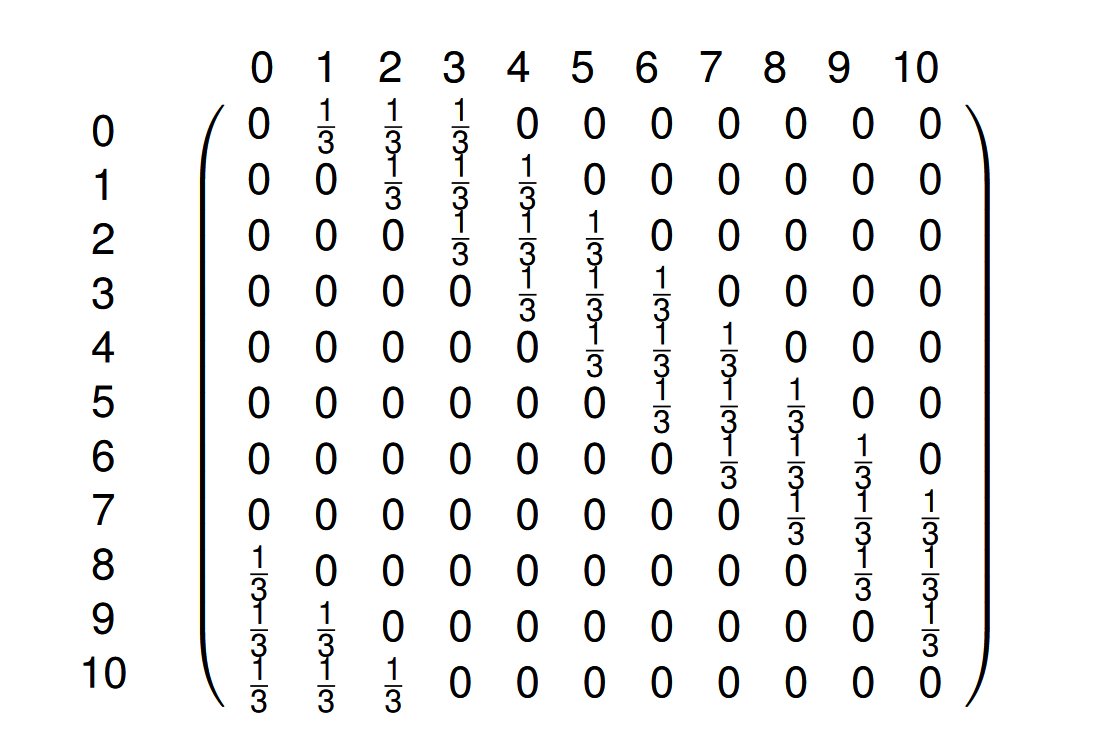
\includegraphics[width=0.4\linewidth]{2.png}
\end{center}

得到一个对称信道,在这种情况下,
$$
H(Y \mid X)=H(Z \mid X)=H(Z)=\left(\frac{1}{3} \log 3+\frac{1}{3} \log 3+\frac{1}{3} \log 3\right) =\log 3,
$$
与$ X $的分布无关,因此信道的容量为
$$
\begin{aligned}
C  =\max _{p(x)} I(X ; Y) & =\max _{p(x)} H(Y)-H(Y \mid X) \\
& =\max _{p(x)} H(Y)-\log 3 \\
& =\log 11-\log 3= \log \frac{11}{3}
\end{aligned}
$$

(2) 当$ Y $具有均匀分布时达到最大值,根据对称性知道, 这发生在$ X $具有均匀分布时,即
$$
p(X)=\frac{1}{11}, \quad, X \in\{0,1, \cdots, 10\} .
$$



\end{tcolorbox}




\begin{tcolorbox}[breakable,colback=blue!5!white,colframe=blue!75!black,
 title= 解答题]

写出二元对称信道, 二元擦除信道及 $ M $ 信道的信道矩阵.
\tcblower

    \centering
    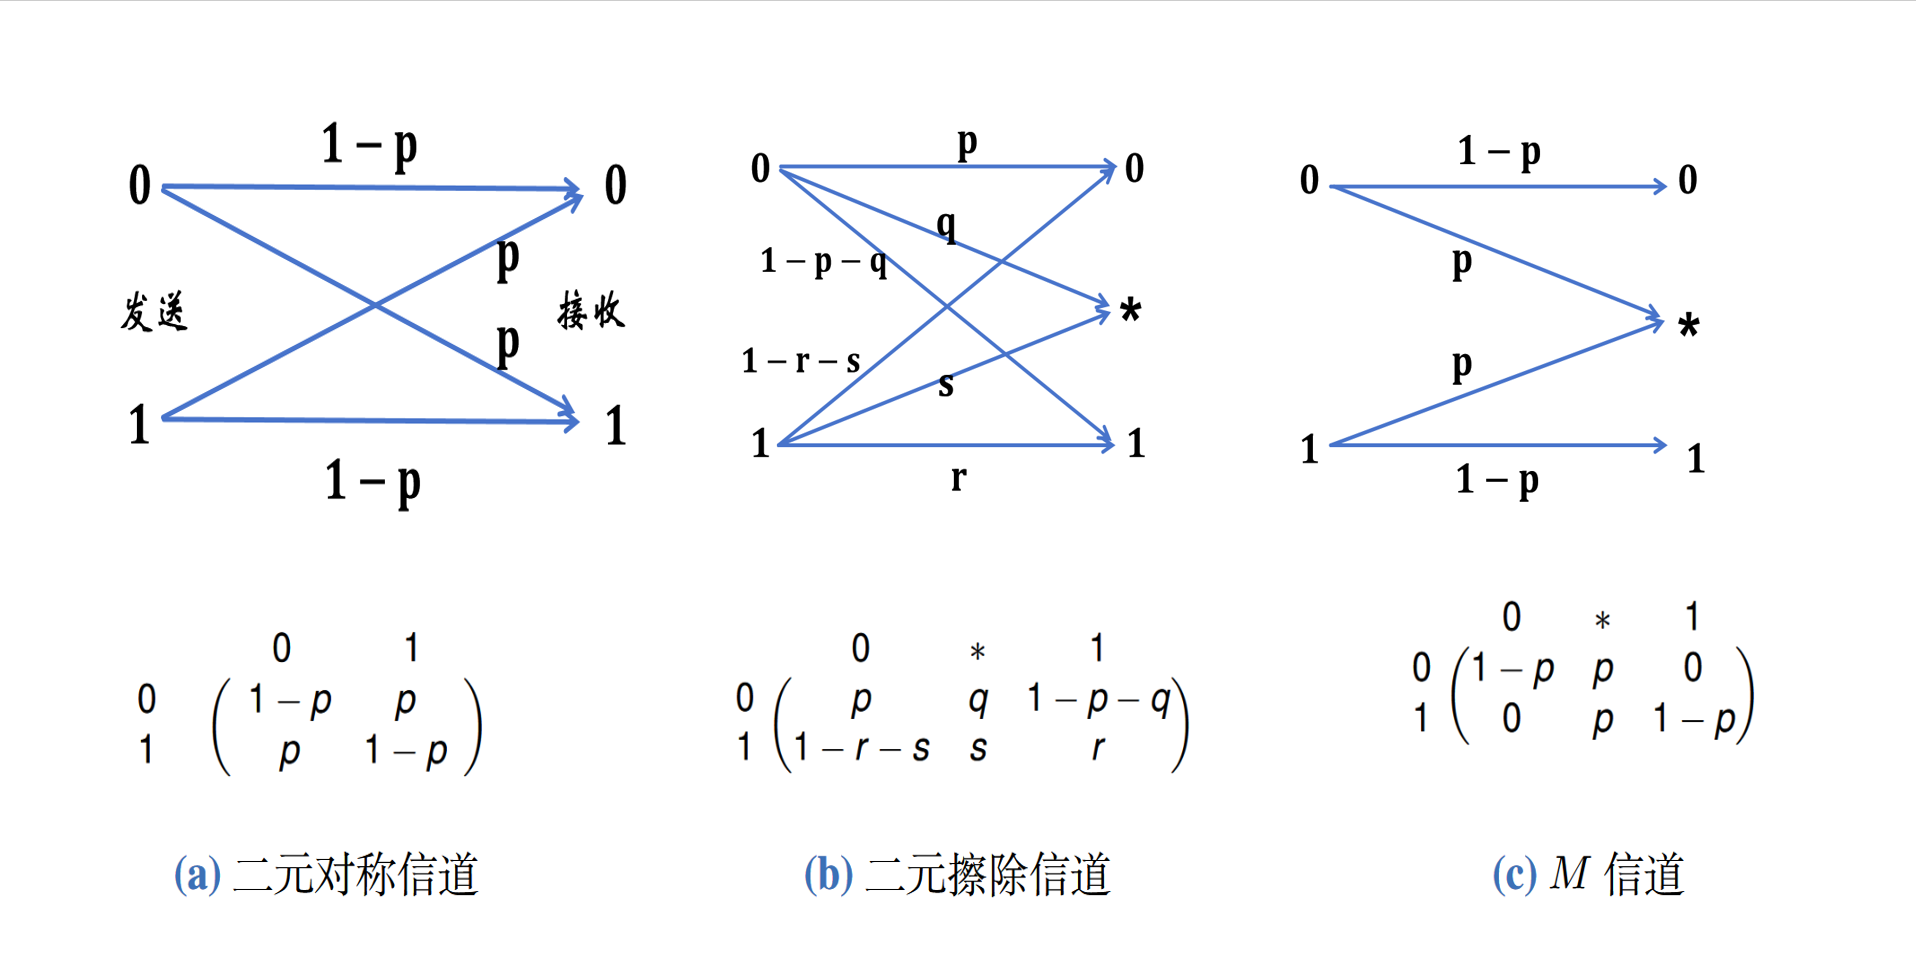
\includegraphics[width=1\linewidth]{3.png}
    
\end{tcolorbox}



